% Copyright 2004 by Till Tantau <tantau@users.sourceforge.net>.
%
% In principle, this file can be redistributed and/or modified under
% the terms of the GNU Public License, version 2.
%
% However, this file is supposed to be a template to be modified
% for your own needs. For this reason, if you use this file as a
% template and not specifically distribute it as part of a another
% package/program, I grant the extra permission to freely copy and
% modify this file as you see fit and even to delete this copyright
% notice. 

\documentclass{beamer}

% There are many different themes available for Beamer. A comprehensive
% list with examples is given here:
% http://deic.uab.es/~iblanes/beamer_gallery/index_by_theme.html
% You can uncomment the themes below if you would like to use a different
% one:
%\usetheme{AnnArbor}
%\usetheme{Antibes}
%\usetheme{Bergen}
%\usetheme{Berkeley}
%\usetheme{Berlin}
%\usetheme{Boadilla}
%\usetheme{boxes}
%\usetheme{CambridgeUS}
%\usetheme{Copenhagen}
%\usetheme{Darmstadt}
%\usetheme{default}
%\usetheme{Frankfurt}
%\usetheme{Goettingen}
%\usetheme{Hannover}
%\usetheme{Ilmenau}
%\usetheme{JuanLesPins}
%\usetheme{Luebeck}
\usetheme{Madrid}
%\usetheme{Malmoe}
%\usetheme{Marburg}
%\usetheme{Montpellier}
%\usetheme{PaloAlto}
%\usetheme{Pittsburgh}
%\usetheme{Rochester}
%\usetheme{Singapore}
%\usetheme{Szeged}
%\usetheme{Warsaw}


% Customize Warsaw color 
\setbeamercolor*{palette primary}{use=structure,fg=white,bg=red!50!black}
\setbeamercolor*{palette secondary}{use=structure,fg=white,bg=red!60!black}
\setbeamercolor*{palette tertiary}{use=structure,fg=white,bg=red!70!black}

% Customize Warsaw block title and background colors
\setbeamercolor{block title}{bg=red!50!black,fg=white}


% List your packages here

\usepackage[colorinlistoftodos]{todonotes}
\usepackage{pgfgantt}


\title[Design Proposal]{Cleaning, Mapping, and Disinfecting Robot Design Proposal}

% % A subtitle is optional and this may be deleted
% \subtitle{Product Proposal}

\author[B.~Lauer]{Brian~Lauer\\\and
Advisors: Dr. Suruz Miah}
% - Give the names in the same order as the appear in the paper.
% - Use the \inst{?} command only if the authors have different
%   affiliation.

\institute[Bradley University] % (optional, but mostly needed)
{
  Department of Electrical and Computer Engineering\\
  Bradley University\\
  1501 W. Bradley Avenue\\
  Peoria, IL, 61625, USA
}
% - Use the \inst command only if there are several affiliations.
% - Keep it simple, no one is interested in your street address.

\date[August~17,~2020]{Monday, August~17,~2020}
% - Either use conference name or its abbreviation.
% - Not really informative to the audience, more for people (including
%   yourself) who are reading the slides online

\logo{\hfill\href{http://www.bradley.edu}{
\includegraphics[width=0.75cm]{figs/logoBU1-Print}}}  % place logo in every page 


\subject{Mobile Robot Localization}
% This is only inserted into the PDF information catalog. Can be left
% out. 

% If you have a file called "university-logo-filename.xxx", where xxx
% is a graphic format that can be processed by latex or pdflatex,
% resp., then you can add a logo as follows:

% \pgfdeclareimage[height=0.5cm]{university-logo}{university-logo-filename}
% \logo{\pgfuseimage{university-logo}}

% Delete this, if you do not want the table of contents to pop up at
% the beginning of each subsection:
% \AtBeginSubsection[]
% {
%   \begin{frame}<beamer>{Outline}
%     \tableofcontents[currentsection,currentsubsection]
%   \end{frame}
% }




% Let's get started
\begin{document}

\begin{frame}
  \titlepage
\end{frame}

\begin{frame}{Outline}
  \tableofcontents
  % You might wish to add the option [pausesections]
\end{frame}

\section{Introduction}
\begin{frame}{Introduction}{}
\begin{figure}
	\centering
	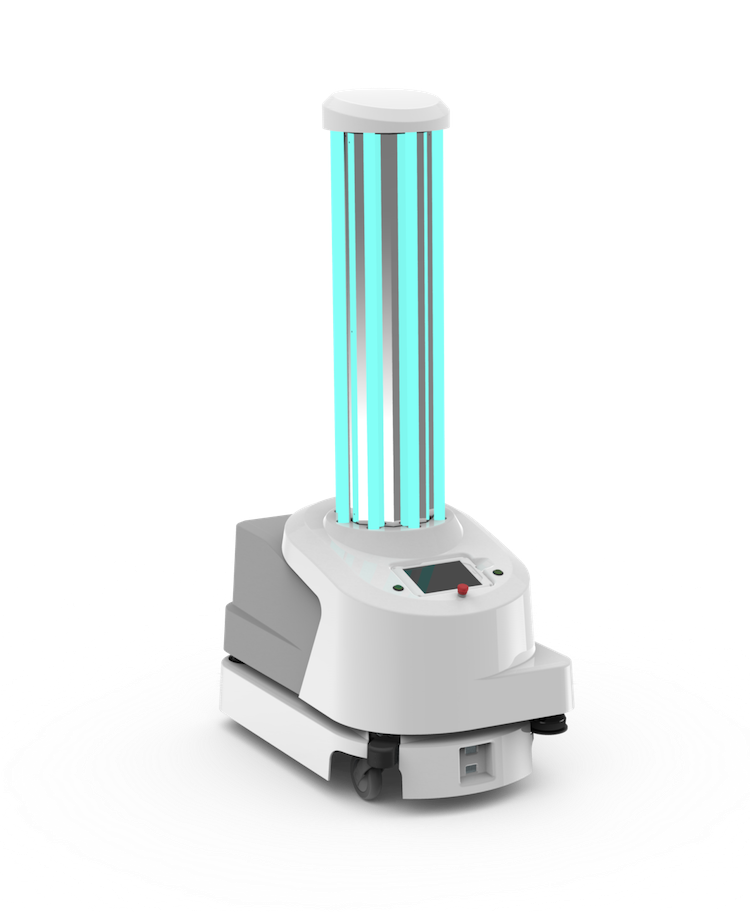
\includegraphics[scale=0.2]{figs/img/UVDR-front}
	\caption{UVD Robot, source: http://www.uvd-robots.com/}
\end{figure}
\end{frame}

\begin{frame}{Introduction}{}
\begin{figure}
	\centering
	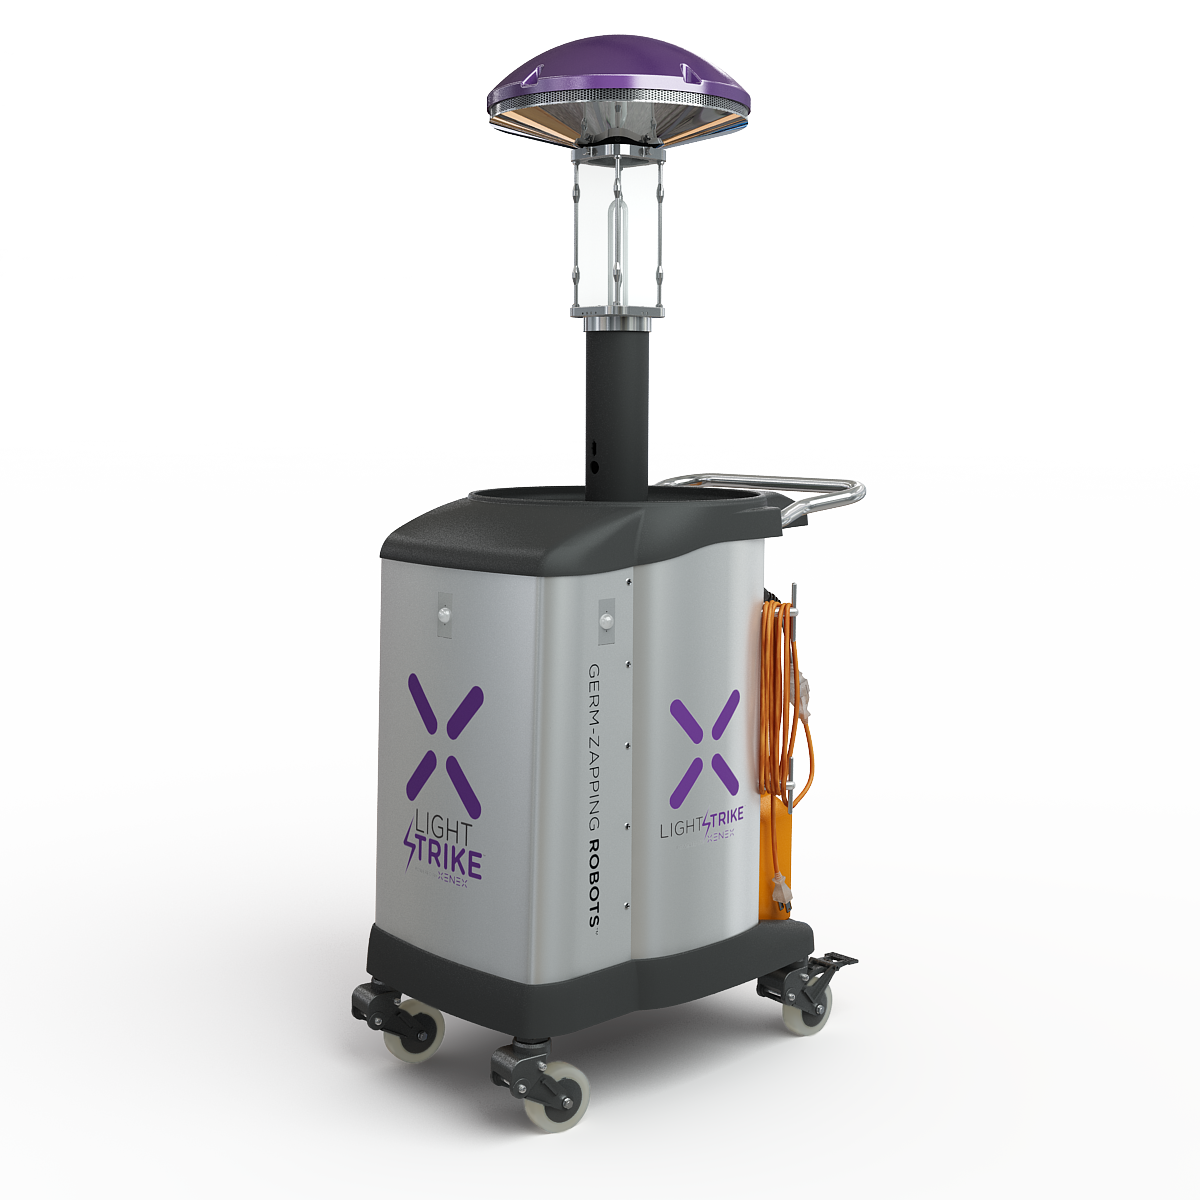
\includegraphics[scale=0.15]{figs/img/xenexLightstrike}
	\caption{Xenex LightStrike Germ-Zapping Robot, source: https://www.xenex.com/our-solution/lightstrike/}
\end{figure}
\end{frame}

\begin{frame}{Proposed Robot Design}
  \begin{exampleblock}{Key Features}
    \begin{itemize}
    \item Proposed robot will offer a modular design and open source architecture
    \item Design will follow plug-and-play architecture -- Disassembly will be one of the key features allowing parts to be added or changed
    \item Software and hardware will follow open-source platform architecture 
      
    \item Proposed robot design will be cost-effective in terms of executing
      navigation algorithms  
    \end{itemize}
  \end{exampleblock}
  \pause
  \begin{exampleblock}{}
    \begin{itemize}
    \item Robot will include a disinfectant sprayer in case a room is unsafe to be cleansed with UV light
    \item Vacuuming feature will be added to further set the robot apart from its commercial counter parts
    \end{itemize}
  \end{exampleblock}
\end{frame}

\section{Current Design}
\begin{frame}{Current Design}{}
\begin{figure}
    \centering
    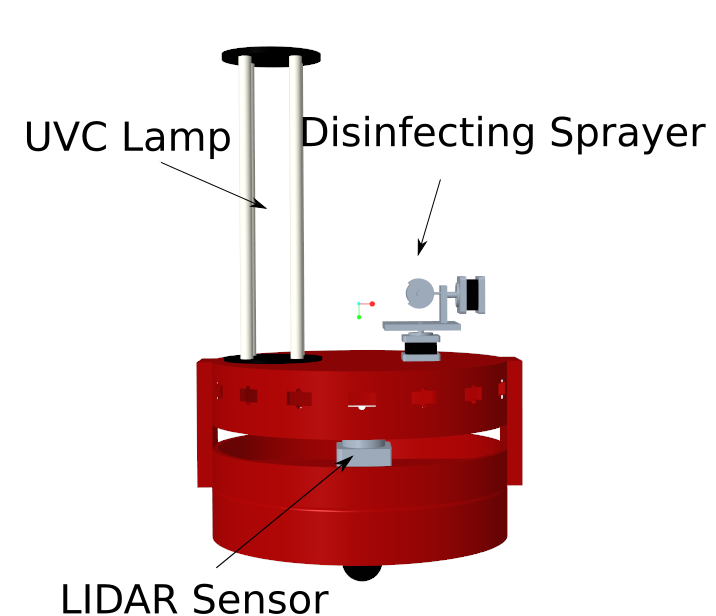
\includegraphics[scale=0.3]{figs/img/frontViewScreenshotA}
    \caption{Side view of the current robot design}
    \label{fig:sideViewRobot}
\end{figure}
\end{frame}

\begin{frame}{Current Design}{}
\begin{figure}
	\centering
	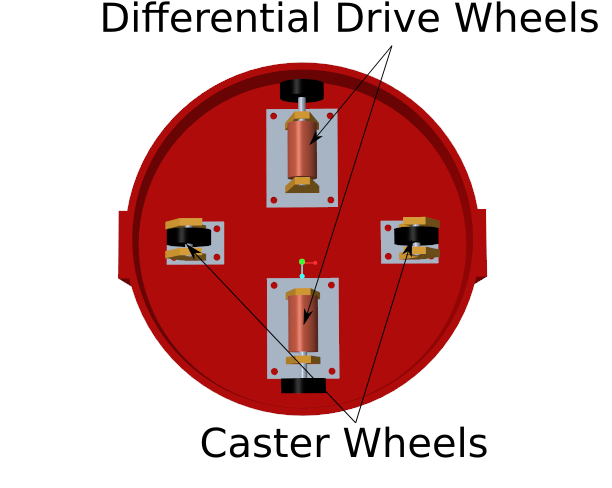
\includegraphics[scale=0.3]{figs/img/bottomViewScreenshotA}
	\caption{Bottom view of the current robot design}
	\label{fig:bottomViewRobot}
\end{figure}

\end{frame}

\section{Development Plan}
\subsection{CAD Modeling}

\begin{frame}{Development Plan}{CAD Modeling}
\begin{ganttchart}[
		hgrid,
		vgrid,
		time slot format=isodate-yearmonth,
		time slot unit=month
	]{2020-07}{2021-2}
%	\gantttitle{2020}{6} \\
%	\gantttitlelist{7,...,12}{1} \\
	\gantttitlecalendar{year,month}\\
	\ganttbar{Redesign outer shell of the robot}{2020-08}{2020-09} \\
	\ganttlinkedbar{Design vacuuming system}{2020-09}{2020-10} \ganttnewline
	\ganttlinkedbar{Create mount points for sensors}{2020-10}{2020-11} \ganttnewline
	\ganttlinkedbar{Design disinfectant sprayer mechanism}{2020-11}{2020-12} \ganttnewline
	\ganttlinkedbar{Design caster and drive wheel mounts}{2020-12}{2021-01}
\end{ganttchart}
\end{frame}

\subsection{Electrical and Software Design}
\begin{frame}{Development Plan}{Electrical and Software Design}
\begin{ganttchart}[
		hgrid,
		vgrid,
		time slot format=isodate-yearmonth,
		time slot unit=month
	]{2020-11}{2021-05}
	\gantttitlecalendar{year,month}\\
	\ganttbar{Develop power delivery system}{2021-01}{2021-02} \\
	\ganttlinkedbar{Create connections with the onboard SBC}{2021-02}{2021-03} \ganttnewline
	\ganttlinkedbar{Develop software and firmware}{2021-03}{2021-04}
\end{ganttchart}
\end{frame}

%% All of the following is optional and typically not needed. 
%\appendix
%\section<presentation>*{\appendixname}
%\subsection<presentation>*{For Further Reading}
%
%\begin{frame}[allowframebreaks]
%  \frametitle<presentation>{References}
%    
%  \begin{thebibliography}{10}
%    
%  \setbeamertemplate{bibliography item}[online]
%  
%  \bibitem{ieeespec}
%  Autonomous Robots Are Helping Kill Coronavirus in Hospitals
%  \newblock \texttt{https://spectrum.ieee.org/automaton/robotics/
%  medical-robots/autonomous-robots-are-helping-kill-
%  coronavirus-in-hospitals}
%
%	\end{thebibliography}
%\end{frame}

\begin{frame}{}{}
\Huge
\centering
\begin{block}{}
  \begin{center}
    Any Questions?
  \end{center}
\end{block}
\end{frame}

\end{document}



%%% Local Variables:
%%% mode: latex
%%% TeX-master: t
%%% End: